%
% File acl2015.tex
%
% Contact: car@ir.hit.edu.cn, gdzhou@suda.edu.cn
%%
%% Based on the style files for ACL-2014, which were, in turn,
%% Based on the style files for ACL-2013, which were, in turn,
%% Based on the style files for ACL-2012, which were, in turn,
%% based on the style files for ACL-2011, which were, in turn, 
%% based on the style files for ACL-2010, which were, in turn, 
%% based on the style files for ACL-IJCNLP-2009, which were, in turn,
%% based on the style files for EACL-2009 and IJCNLP-2008...

%% Based on the style files for EACL 2006 by 
%%e.agirre@ehu.es or Sergi.Balari@uab.es
%% and that of ACL 08 by Joakim Nivre and Noah Smith

\documentclass[11pt]{article}
\usepackage{acl2015}
\usepackage{times}
%\usepackage{url}
\usepackage{latexsym}
\usepackage{amsmath}
\usepackage{enumitem}
\usepackage[usenames, dvipsnames]{color}
\setlist{nosep}
\usepackage[round]{natbib}
\usepackage[export]{adjustbox}% http://ctan.org/pkg/adjustbox
\usepackage{amsfonts}
\usepackage{tabularx} % in the preamble
\usepackage[hyphens]{url}

\newtheorem{definition}{Definition}
\DeclareMathOperator*{\argmax}{arg\,max}
%\setlength\titlebox{5cm}

% You can expand the titlebox if you need extra space
% to show all the authors. Please do not make the titlebox
% smaller than 5cm (the original size); we will check this
% in the camera-ready version and ask you to change it back.


\title{R222 Assignment}

\author{Kaho Sato \\
King's College \\
  {\tt ks789@cam.ac.uk}}

\date{}

\begin{document}
\maketitle
%\begin{abstract}
%\end{abstract}

\section{Introduction}
\label{sec:introduction}
There is an increasing interest in Native Language Identification (NLI).
Native Language Identification involves detecting the native language (L1) of the author of the text.
This is a sub-task of author profiling, where the goal is to predict traits of the author such as gender, age or psychometric traits \citep{estival2007author}.
Author profiling has been used to combat the criminal activity\citep{abbasi2005applying} to gain an insight to the suspects by analysing the online mediums used for communication among them.
 q 		

\section{Related Work}
\label{sec:related_work}
The first work on NLI that we are aware of is that of \cite{koppel2005determining}.
They used SVM to perform five-class classification between Russian, Czech, Bulgarian, French, and Spanish.
The features they extracted include stylistic features such as function words, character n-grams, and grammatical errors.
They report the accuracy of 80.2\%.
\cite{tsur2007using} performs the exact same task using SVM and investigates the effect of each features used.
\cite{wong2011exploiting} experiment with substructures of a parse tree as additional features and achieve the accuracy of 80\% in seven-class classification with SVM.
\cite{swanson2012native} also used SVM and fragments of Tree Substitutional Grammar as additional features. This gave 78.4\% accuracy in the same task as \cite{wong2011exploiting}.
\cite{swanson2012native} replicate the work by \cite{wong2011exploiting} and report the accuracy of 72.6\%.

Aside from SVM, Latent Dirichlet Analysis was applied to NLI with seven languages by \cite{dras2011topic}.
This gave the accuracy of 56.9 \%, which was lower than 64.1\% accuracy that their baseline SVM gave.
All the works mentioned up to this point uses the ICLE corpus \citep{granger2002international}.

In 2013, the First Native Language Identification Shared Task was held \citep{tetreault2013report}.
The task was to perform NLI on the new TOEFL11 corpus \citep{tetreault2013report} which included essays written by native speakers of 11 languages.

As mentioned previously, the majority, including the winning team  \citep{jarvis2013maximizing}, utilised SVM.
\cite{jarvis2013maximizing} achieves the accuracy of 83.6\%.

The other approaches seen in the shared task include MaxEnt, Ensemble, and Discriminant Function Analysis \citep{tetreault2013report}.



\section{Background}
\label{sec:background}
In this section, we describe one dimensional CNNs which are commonly used in natural language processing\citep{collobert2008unified, collobert2011natural, kalchbrenner2014convolutional, zhang2015character, goldberg2016primer}.

CNNs are made up of two parts; convolutional layers and fully-connected layers.
The role of convolutional layers is to produce the most salient information of the input \citep{goldberg2016primer}.
The output of the convolutional layers are then fed to the fully-connected layers, which perform the prediction.
We omit the description of fully-connected layers.

A convolutional layer applies three operations to its input.
The first operation is \emph{convolution}, which is the application of a linear function to a window of the input. 
The window is moved with some stride, and the convolution is applied to each window \citep{goldberg2016primer}.
%In convolution, a function is applied to a region of the input 
%In this section we describe the \emph{temporal convolution}.
%When a CNN takes images as an input, the convolution is applied in two dimension.
%Let the dimension of the input layer to be $m_i \times n_i$.
%In two dimensional convolution, the size of kernel, say $m_k \times n_k$ is such that $m_k < m_i$ and $n_k < n_i$, and the kernel is ``moved'' to both directions.
%
%In temporal convolution, which is often used in natural language processing, the convolution is applied in a single dimension.
%Each feature, a character in this report, is represented as a vector of length $m_i$ and $n_i$ of them constitute the input.
%In one dimensional convolution, the size of kernel is such that $m_k = m_i$ and the kernel is moved along the column.
Let $l$ be the number of the features which represent the input, and $k$ be the width of the sliding window.
Let $f(x)$ be a function which takes an index in the window $x \in [1, k]$ and returns the weight applied to the $x$th element.
Let $g(x)$ be a function which takes an index of the input $x \in [1, l]$ and returns the $x$th feature in the input.
Let $d$ be the stride of the convolution.
Then, the result of the convolution applied to $y$th window is expressed as the following function $h(y)$ \citep{zhang2015character}:
\begin{align*}
h(y) = \sum_{x=1}^{k} f(x) \cdot g(y \cdot d - x + c)
\end{align*}
where $c = k - d + 1$ is an offset constant.

The second operation is \emph{non-linearlity} which is applied to each result of the convolution.
This allows CNNs to model a non-linear function.
A popular choice of non-linearlity is \emph{rectifier}, defined as:
\begin{align*}
ReLU(x) = max(0, x)
\end{align*}

The last operation in a convolutional layer is \emph{pooling}.
Similarly to convolution, the pooling operation is also done with a sliding window, moved with a certain stride.
In pooling, the information in the window is aggregated by some function.
For instance, in max-pooling, the function returns the largest element in the window is used.
Another popular function for pooling returns the average of the elements in the window.
The purpose of pooling is to reduce the to possibility of overfitting by downsizing the input and reducing the number of parameters in the later layers \citep{krizhevsky2012imagenet}.

In the training, the loss is calculated from the output of the fully-connected network, and the error gradients are propagated back to the convolutional layers to adjust the weight applied by $f(x)$ in convolution \citep{goldberg2016primer}.
Thus the features that the convolutional layers extract from the input are most informative for the particular prediction task the network is trained for.


\section{Dataset}
\label{sec:dataset}
We use a subset of the Cambridge Learner Corpus \citep{nicholls2003cambridge} (CLC).
CLC is a corpus which consists of scripts produced by learners with 86 different L1 for various Cambridge English Language Assessment examinations.
Each document is annotated with basic information of the author, such as their L1 and age, making CLC appropriate corpus for author profiling.

In particular, we use a subset of the publicly available CLC FCE Dataset \citep{yannakoudakis2011new} as a test set.
This contains 1244 scripts, each containing two answers, produced by learners with 16 different L1 for the Cambridge ESOL First Certificate in English (FCE) examination in 2010 and 2011.

Table \ref{tab:l1-fce} shows the number of scripts for each L1 in the CLC FCE Dataset.
\begin{table}[]
\centering
\caption{Distribution of L1 in the CLC FCE Dataset}
\label{tab:l1-fce}
\begin{tabular}{|c|c|}
\hline
L1         & Count \\ \hline
Dutch      & 2     \\ \hline
Swedish    & 15    \\ \hline
Thai       & 63    \\ \hline
Catalan    & 64    \\ \hline
Chinese    & 66    \\ \hline
Portuguese & 68    \\ \hline
German     & 69    \\ \hline
Greek      & 74    \\ \hline
Italian    & 76    \\ \hline
Polish     & 76    \\ \hline
Turkish    & 77    \\ \hline
Japanese   & 80    \\ \hline
Russian    & 82    \\ \hline
Korean     & 86    \\ \hline
French     & 146   \\ \hline
Spanish    & 200   \\ \hline
\end{tabular}
\end{table}
We extracted scripts produced by Japanese, Russian, and Italian native speakers to create a test set of 476 examples (Recall that each script contains two answers).
We chose these three languages for two reasons;
Firstly, the number of the scripts available for each language is fairly even.
Secondly, they belong to the separate language families, which should make the classification more manageable.
We selected 3000 answers from the CLC, 1000 for each L1, to build a training set.

The level of proficiency is another variable that influences the writing of a learner, and this may introduce an undesirable bias.
Each Cambridge ESOL examination expects a certain level of proficiency from the candidates.
The reference levels are provided by Common European Framework of Reference for Languages (CEFR) \citep{council2001common}, and FCE is aimed for learners at CEFR level B (i.e. independent user).
For the training set, for each language, we selected 250 answers by learners at CEFR level A and C (i.e. basic and proficient user, respectively) and 500 answers by learners at CEFR level B.
We included more answers produced by learners at CEFR level B in order to assimilate the training set to the test set.
Besides, it is reasonable to assume that there are more independent users than basic or proficient users.

Table \ref{tab:tr-stat} and \ref{tab:te-stat} gives the statistic of the character counts of the documents in the training and test set respectively.
As can be seen, there is a much larger variance in the training set than in the test set.
This is due to the fact that the training set contains answers for 15 different exams, where the expected length of the answers is different from one another, whereas the test set only contains answers for FCE.
\begin{table}[h]
\centering
\caption{Statistics of the Character Length of Documents in Training Set}
\label{tab:tr-stat}
\begin{tabular}{|c|c|}
\hline
Min         & 58 \\ \hline
Max      & 3710     \\ \hline
Median    & 376.5    \\ \hline
Average & 742.1   \\ \hline
Standard Deviation    & 716.4   \\ \hline
\end{tabular}
\end{table}
\begin{table}[h]
\centering
\caption{Statistics of the Character Length of Documents in Test Set}
\label{tab:te-stat}
\begin{tabular}{|c|c|}
\hline
Min         & 685\\ \hline
Max      & 1822     \\ \hline
Median    & 1081   \\ \hline
Average & 1099    \\ \hline
Standard Deviation    & 186.8    \\ \hline
\end{tabular}
\end{table}

From the training set, we took 300 examples to create a validation set.
The error rate on the validation set is computed after each epoch and was used to see the length of training which does not make the model to underfit or overfit to the remaining 2700 examples.


\section{Architecture}
\label{sec:architecture}
We use the CNN described in \citep{zhang2015character}.
The implementation is based on Torch \citep{torch} and available online\footnote{\url{https://github.com/zhangxiangxiao/Crepe}}.
In this section, we describe their design and the modifications we experimented with.
\subsection{Input}
\label{sub:input}
We first need to encode documents to a fixed sized sequence of vectors, so it can be fed to the temporal convolutional module described in Section \ref{sec:background}.
\cite{zhang2015character} do this by lowercasing the document, and mapping each character to a one-hot vector.
The alphabet used in our experiment is the same as in \citep{zhang2015character} and is 
\begin{verbatim}
abcdefghijklmnopqrstuvwxyz
0123456789
-,;.!?:’"/\|_@#$%ˆ&*˜‘+-=<>()[]{}
\end{verbatim} 
As the alphabet consists of 70 characters, each document is transformed into a sequence of vectors of size 70.
If a character in a document is not present in the alphabet, it is encoded to an all-zero vector.
Note that a whitespace is not part of the alphabet and therefore is also encoded to an all-zero vector.

\cite{zhang2015character} perform a data augmentation in order to avoid the generalisation error.
Specifically, they use an English thesaurus which is based on WordNet\color{red}cite\color{black} and replace words in the document to create a ``new'' example.
The number of words to be replaced and the index of the synonym used is chosen probabilistically.
This data augmentation technique is appropriate if the task is to classify the documents according to its semantics.
Indeed, the text classification tasks that \cite{zhang2015character} use this CNN for are sentiment analysis and topic classification.
Though the dataset we have is small and a data augmentation would have been useful, it was expected that this particular technique would introduce an undesirable noise in training for author profiling, as word choice is a crucial cue for the attributes of the author, especially their L1.
\cite{yarowsky2013learning} shows that the frequency distribution of words used in a corpus of computational linguistics articles from the ACL Anthology varies greatly from L1 to L1 of the author.
For instance, a word ``claim'' is much less often used by Chinese native speakers than native speakers of other languages, and ``complementary'' is more frequently used by French or Spanish native speakers.
The latter can potentially be explained by the latin origin of the word.
To preserve such distinguishing features in the data, we turned off the data augmentation.

In \citep{zhang2015character}, the first 1014 characters are taken from each document and encoded to be used as an input.
This is potentially problematic with the dataset we have.
As shown in \color{red} CREATE TABLE AND REFERENCE HERE \color{black}, majority of the documents in the training set is significantly shorter than 1014 characters.
Though pooling should help the model to be invariant to the location of a feature, having majority of the training examples padded extensively might be harmful.

To partially mitigate the problem of small dataset and short documents, instead of taking the first 1014 characters, we take a window of smaller size at an arbitrary location.
For instance, given a document of length 1000 and a window size $l_w = 100$, a CNN may sample 100 characters at 900 different locations, effectively creating 900 samples.
In this report, we refer to this approach as \emph{random window sampling}.
We experiment with $l_w \in \{123, 339, 555, 771, 1014\}$.
Note that these numbers are chosen as they are compatible with the architecture.
\subsection{Architecture}
\begin{figure*}[h]
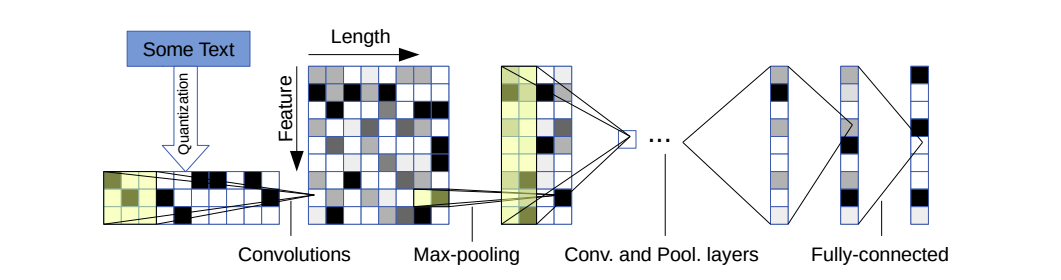
\includegraphics[width=\textwidth]{architecture.png}
\caption{Overview of Architecture}
\label{fig:architecture}
\end{figure*}

Figure \ref{fig:architecture} gives an illustration of the model described in \citep{zhang2015character}.
The CNN consists of 6 convolutional, and 3 fully-connected layers.
The kernel described in Section \ref{sub:conv} is applied with stride 1.
The activation function used is a threshold function $th$ defined as follows:
\[
  th(x) =
  \begin{cases}
    x & \text{if $x > 1\mathrm{e}{-6}$} \\
    0 & \text{otherwise}
  \end{cases}
\]
Max-pooling is applied with stride 3 at first, second and sixth convolutional layer.
Table \ref{tab:conv-config} shows the configuration of the convolutional layers.
\begin{table*}[t]
\centering
\caption{Convolutional Layers Used in \citep{zhang2015character}}
\label{tab:conv-config}
\begin{tabular}{cccc}
Layer & Frame Size & Kernel Width & Pooling Region Width \\ \hline
1     & 256        & 7            & 3                    \\
2     & 256        & 7            & 3                    \\
3     & 256        & 3            & N/A                  \\
4     & 256        & 3            & N/A                  \\
5     & 256        & 3            & N/A                  \\
6     & 256        & 3            & 3                   
\end{tabular}
\end{table*}
The number of features of the input is 70, which is the size of the alphabet given in \ref{sub:input}.
As stated previously, in \citep{zhang2015character} the length of the input is 1014.
With our approach of random window sampling, the length of the input is equal to the window size $l_w$.
The output frame length after the last convolutional layer is $(l_0 - 96) / 27$, where $l_0$ is the length of the input.
This defines a set of possible window sizes $l_w$.

Between the fully-connected layers, dropout modules \citep{hinton2012improving} with dropout probability of 0.5 are used for regularisation.
Seventh and eighth layer have 1024 output units, and ninth layer have three as this is applied to three-class classification.


\section{Results}
\label{sec:results}

\begin{table*}[]
\centering
\caption{Error Rate of Models with Input Size 1014}
\label{tab:1014}
\begin{tabular}{cccc}
& Random Window Sampling & Augmentation  & Error Rate \\ \hline
(A)& No                     & Yes                & 0.648      \\
(B)& No                     & No                 &0.664     \\
(C)& Yes                     & Yes                &  0.640    \\
(D)& Yes                    & No                 & 0.626
\end{tabular}
\end{table*}
Table \ref{tab:1014} shows the error rate of the CNN with the input size 1014.
Model (A) is the unmodified implementation described in \citep{zhang2015character}.
As described in Section \ref{sub:input}, we modify the implementation in two ways; one is applying the random window sampling, and the other is switching off the data augmentation using a thesaurus.

The error rate of a simple baseline system which chooses the label arbitrarily is $0.667$. 
All the models perform better than the baseline though only by a small margin.

As can be seen in the table, (D) outperforms all the other models, showing the effectiveness of the two modifications.
As stated previously, this CNN is shown effective for sentiment analysis and topic categorisation \citep{zhang2015character}.

We argue that random window sampling is an effective data augmentation method for this task.
In \citep{zhang2015character}, the types of documents treated are reviews or articles, and the first part of these documents tend to be more informative about the overall content which is the objective of the network.
Using only the start of the document therefore means less noise in the training data for the problems discussed in \citep{zhang2015character}.
However, in the context of NLI, there is no clear relation between the informative features and the locations.
Therefore it could be useful to augment the small dataset with random window sampling, rather than discarding a possibly useful information which may be contained in the later part of the training example.

A possible explanation of (A) performing better than (B) is that augmentation using thesaurus helps generalise the bias introduced by using only the first part of the document.
The bias may be related to the topic of the document or to the format that the exam prompt asks for.
There is an imbalance in the exams taken by native speakers of each language, and therefore there may be a prompt on a certain topic or asks for a certain format which was chosen more frequently by a learners of a certain L1. 
Clearly, if a network learns to classify based on the topic or the format, it would not generalise and perform poorly on the test set.
As mentioned previously, the first part of the document may contain more information about the topic, and it possibly is more affected by the format.
For instance, there are many documents which are in the format of a letter.
These always start with a greeting (e.g. Dear ...), and if there are more of such documents are present for a certain L1, the network may associate the greeting with this L1, which would not generalise.

\begin{table}[]
\centering
\caption{Error Rate of Models with Random Window Sampling}
\label{tab:r_w_s}
\begin{tabular}{ccc}
&Input Size & Error Rate \\ \hline
(D)&123        & 0.578      \\
(E)&339        & 0.632      \\
(F)&555        & 0.654      \\
(G)&771        & 0.682      \\
(C)&1014       & 0.626    
\end{tabular}
\end{table}
\begin{table}[]
\centering
\caption{Proportion of Examples with Padding}
\label{tab:padding}
\begin{tabular}{ccc}
Input Size & Training & Test \\ \hline
123        & 1.20\%  &   0\% \\
339        & 46.5\%    & 0\%\\
555        & 58.5\%    & 0\% \\
771        & 68.7\%     &2.5\% \\
1014       & 74.3\%    &33.6\%
\end{tabular}
\end{table}
Table \ref{tab:r_w_s} shows the result for a different window size.
Again, all the models except for (G) perform better than the simple baseline system only by small margin.

Interestingly, the best performances were achieved with the smallest and the largest window size.
This suggests that there is a trade-off between a small and a large window.
Intuitively, having a large window would mean that the network is fed with more information, which is beneficial.
It, however, also means that the network is fed with more padding.
Table \ref{tab:padding} shows the proportion of examples which are padded in each dataset.
As can be seen, with a window size larger than 123, a large proportion of the training set is padded.
Though the padding itself potentially introduces some noise, it affected the network less with the window size 1014, perhaps because also many examples in the test set was padded.
As a future work, one may filter short examples which require padding from training set and see whether the performance improves.

A possible explanation to a large difference between the performance of the CNN applied to this task and the tasks introduced in \citep{zhang2015character} is the size of dataset.
The smallest dataset \cite{zhang2015character} experiment with consists of 120k training examples equally split between four classes, which is significantly larger than our dataset.
\cite{zhang2015character} also states that convolutional networks, especially when learning from low-level raw features (i.e. characters).
On the contrary, \cite{stab2017recognizing} uses a convolutional network to classify arguments as sufficient or not.
With just over 1000 examples, the error rate of their network is $0.157 \pm 0.025$, which is much lower than that of the majority baseline, which is $0.338 \pm 0.033$.
This network takes word embeddings produced with word2vec \citep{mikolov2013distributed}.
Though lexical features are not considered to be appropriate for the task of NLI as stated previously, for a future work it may be worth investigating the use of word-based CNN for NLI.

\section{Conclusion}
\label{sec:conclusion}
In this report we investigated whether a CNN designed by \cite{zhang2015character} is effective for NLI.
Though it did perform better the baseline system, the improvement was minuscule. 
We experimented with two modifications to their implementation. One is to switch off the data augmentation using thesaurus, and the other is to use random window sampling.
Each modification alone gave no improvement, but when both were applied the error rate went down by 2.2\%.

We also experimented with a various window sizes, and found that the smallest window size performed the best. This gave an improvement of 8.9\% to the baseline, and 7.0\% to the original implementation by \cite{zhang2015character}.

As no existing work in NLI uses the same dataset, we can not compare the performance directly.
However, a very simple SVM gives a good performance for different corpora, and it is expected that it would outperform any of the models discussed in this report. 

% include your own bib file like this:
\bibliography{r222}
\nocite{*}
\bibliographystyle{plainnat}


\end{document}